\section{Stoppages}

Stoppage represents another concept required for Transporter project users. Stoppage is a small movement of machine during large time on small territory. The stoppage report can show illegal ... 

\begin{figure}[H]
\centering
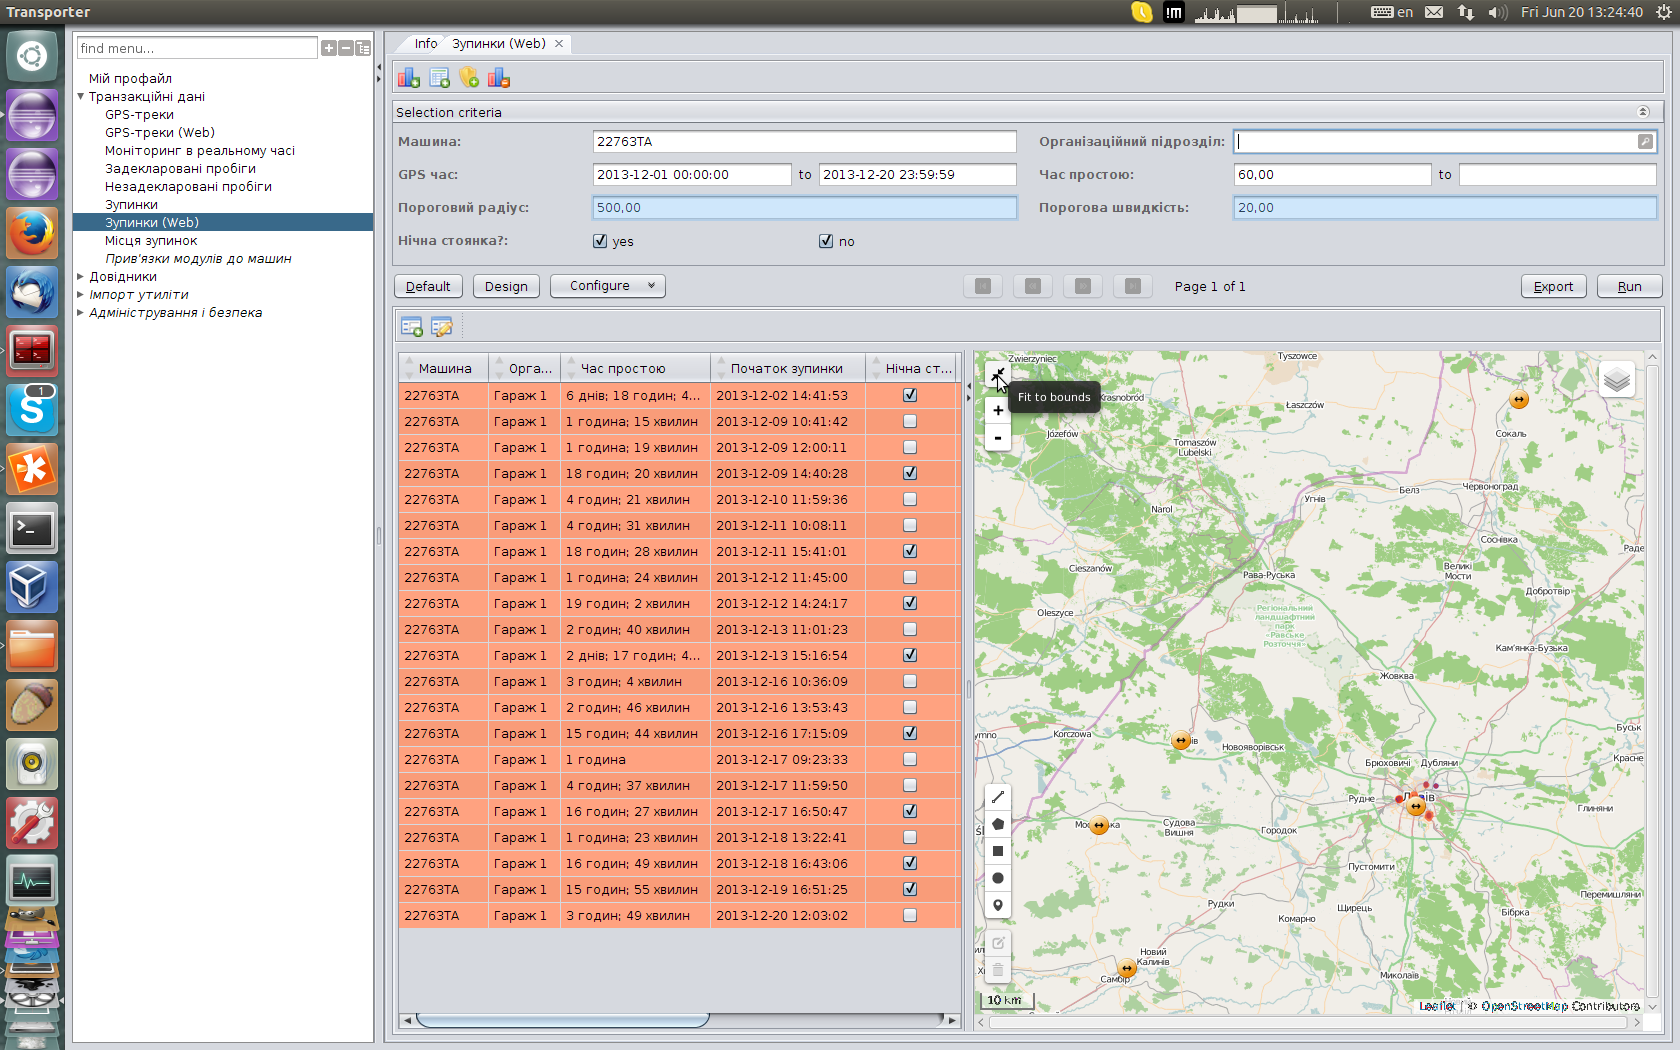
\includegraphics[width=\linewidth]{chapters/03-stoppages/images/21-all-stoppages-using-fit-to-bounds-button.png}
\caption{all-stoppages-using-fit-to-bounds-button}\label{fig:21}
\end{figure}

\begin{figure}[H]
\centering
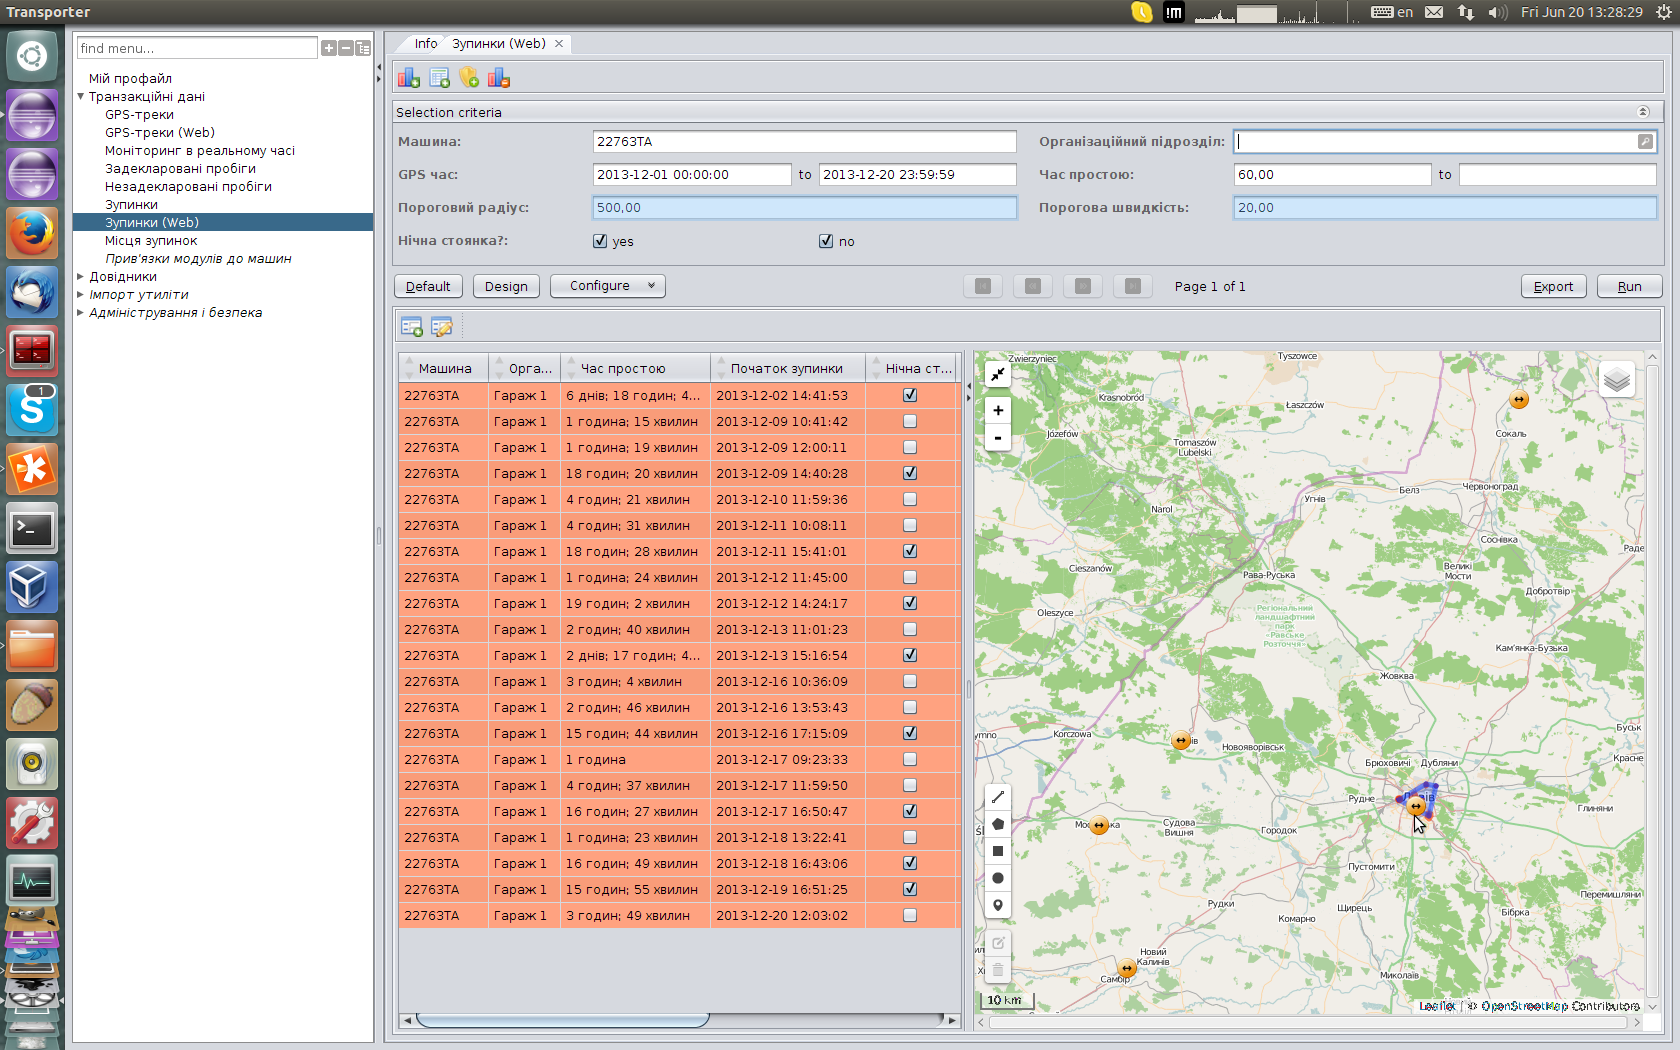
\includegraphics[width=\linewidth]{chapters/03-stoppages/images/22-part-of-stoppages-zooming-by-clicking-cluster-near-lviv.png}
\caption{part-of-stoppages-zooming-by-clicking-cluster-near-lviv}\label{fig:22}
\end{figure}

\begin{figure}[H]
\centering
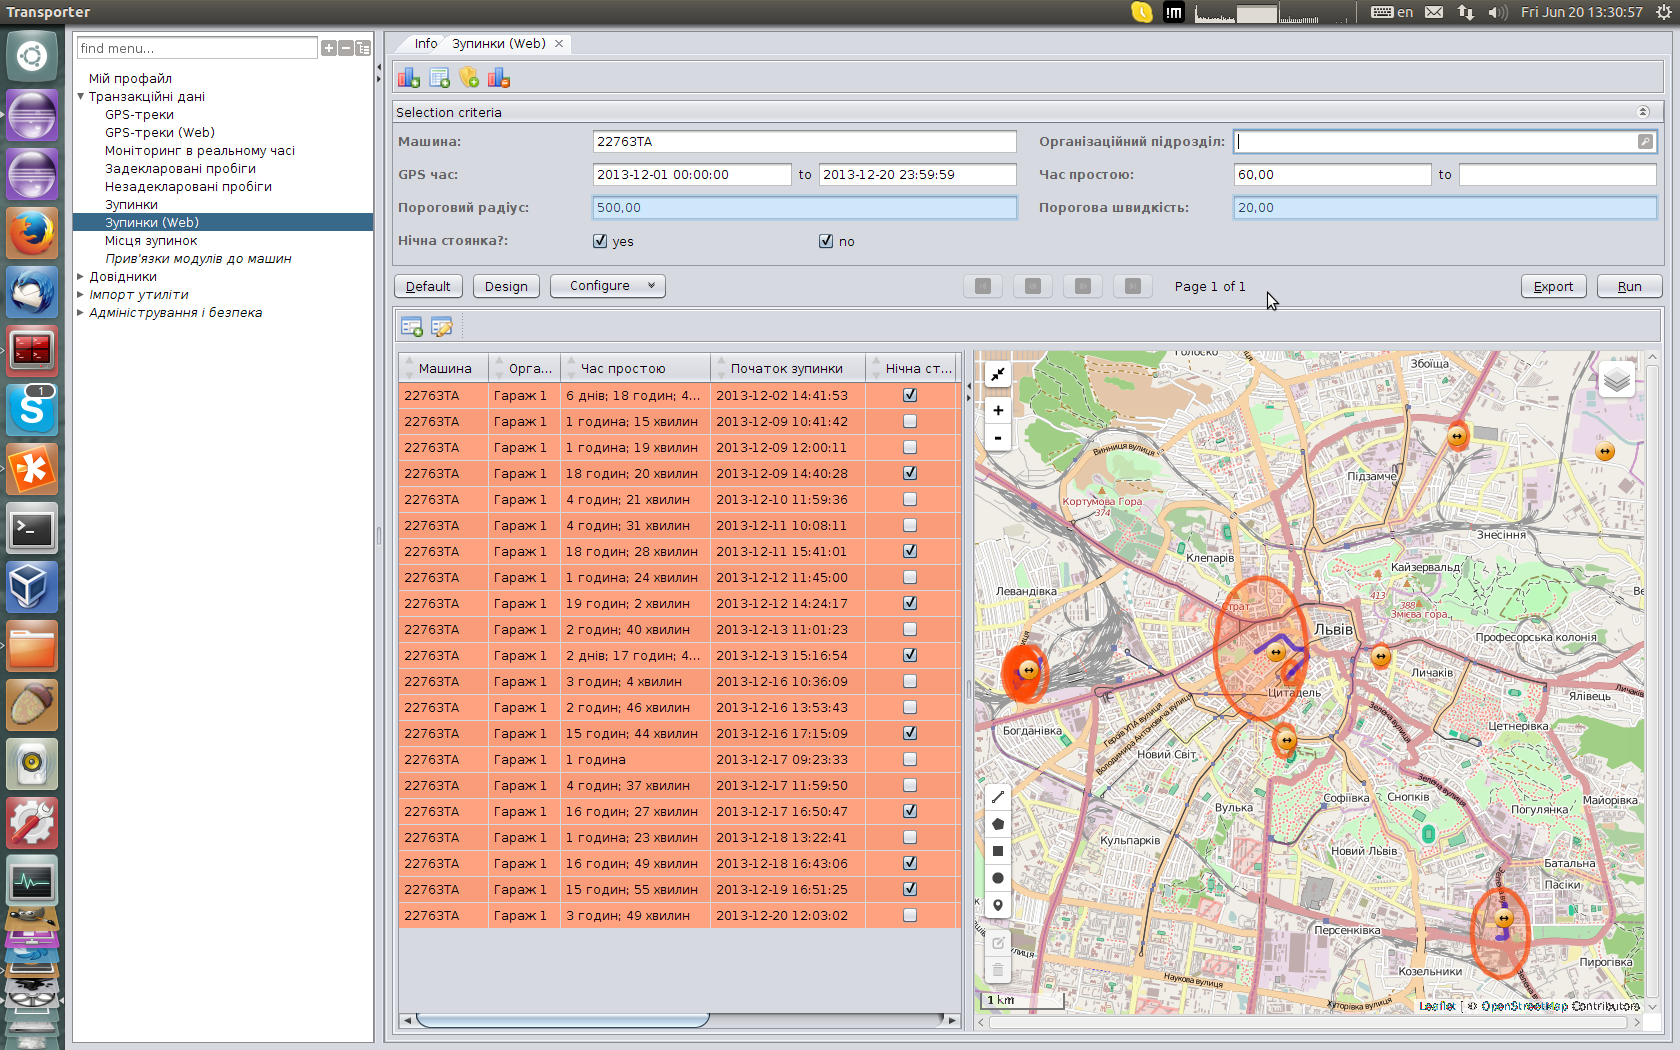
\includegraphics[width=\linewidth]{chapters/03-stoppages/images/23-part-of-stoppages-zoomed-in.png}
\caption{part-of-stoppages-zoomed-in}\label{fig:23}
\end{figure}

\begin{figure}[H]
\centering
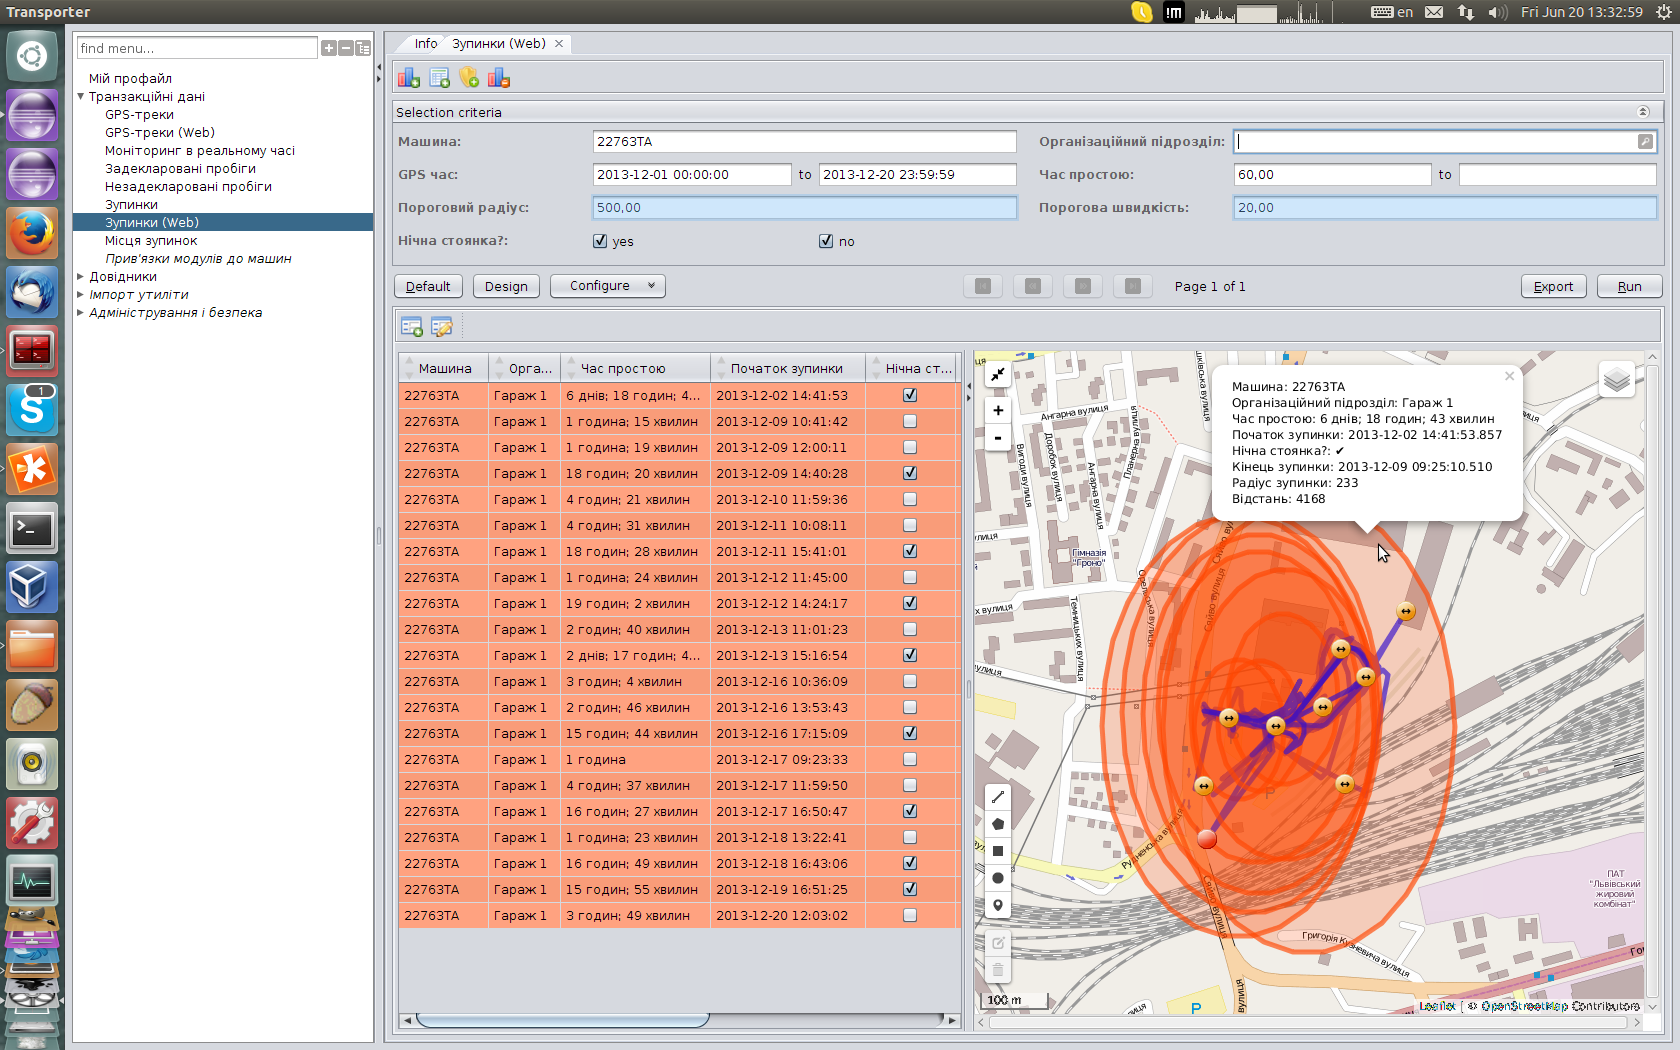
\includegraphics[width=\linewidth]{chapters/03-stoppages/images/24-a-plenty-of-night-stoppages-in-the-same-place-with-one-selected-popup-details.png}
\caption{a-plenty-of-night-stoppages-in-the-same-place-with-one-selected-popup-details}\label{fig:24}
\end{figure}

\begin{figure}[H]
\centering
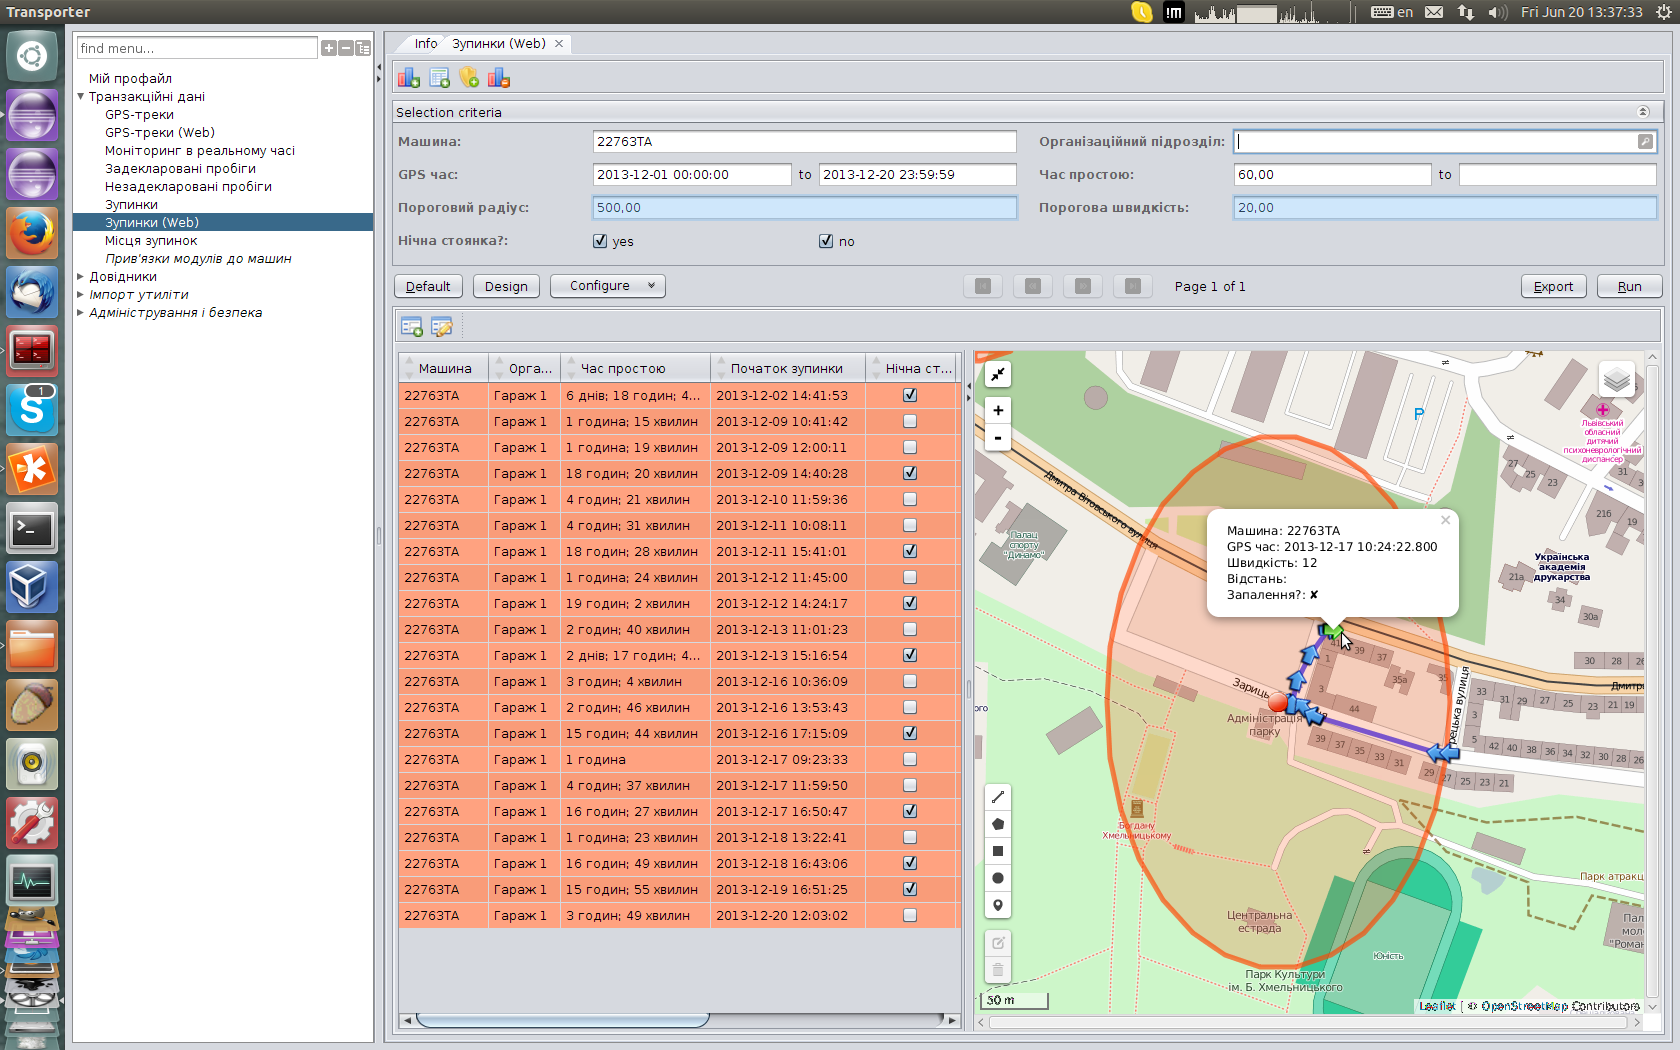
\includegraphics[width=\linewidth]{chapters/03-stoppages/images/25-detailed-stoppage-analysis-by-its-messages.png}
\caption{25-detailed-stoppage-analysis-by-its-messages}\label{fig:25}
\end{figure}

\begin{figure}[H]
\centering
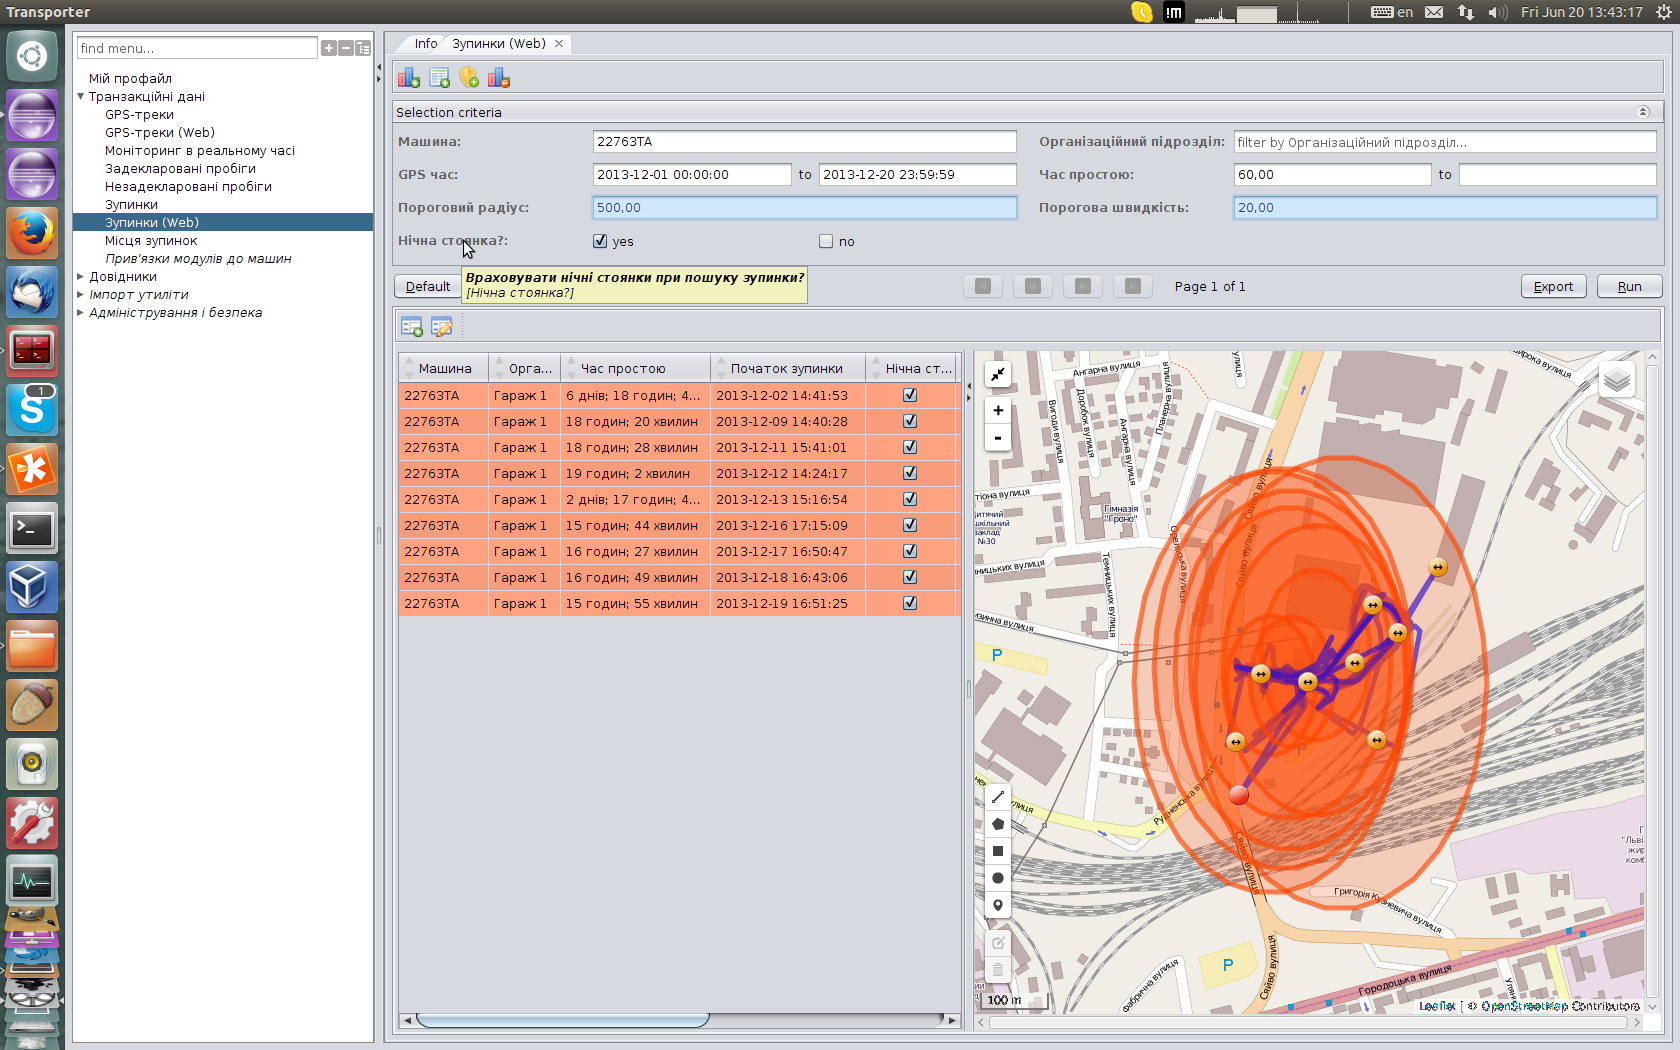
\includegraphics[width=\linewidth]{chapters/03-stoppages/images/26-determining-whether-machine-has-nightstopped-at-base-in-particular-period-of-time.png}
\caption{determining-whether-machine-has-nightstopped-at-base-in-particular-period-of-time}\label{fig:26}
\end{figure}

\begin{figure}[H]
\centering
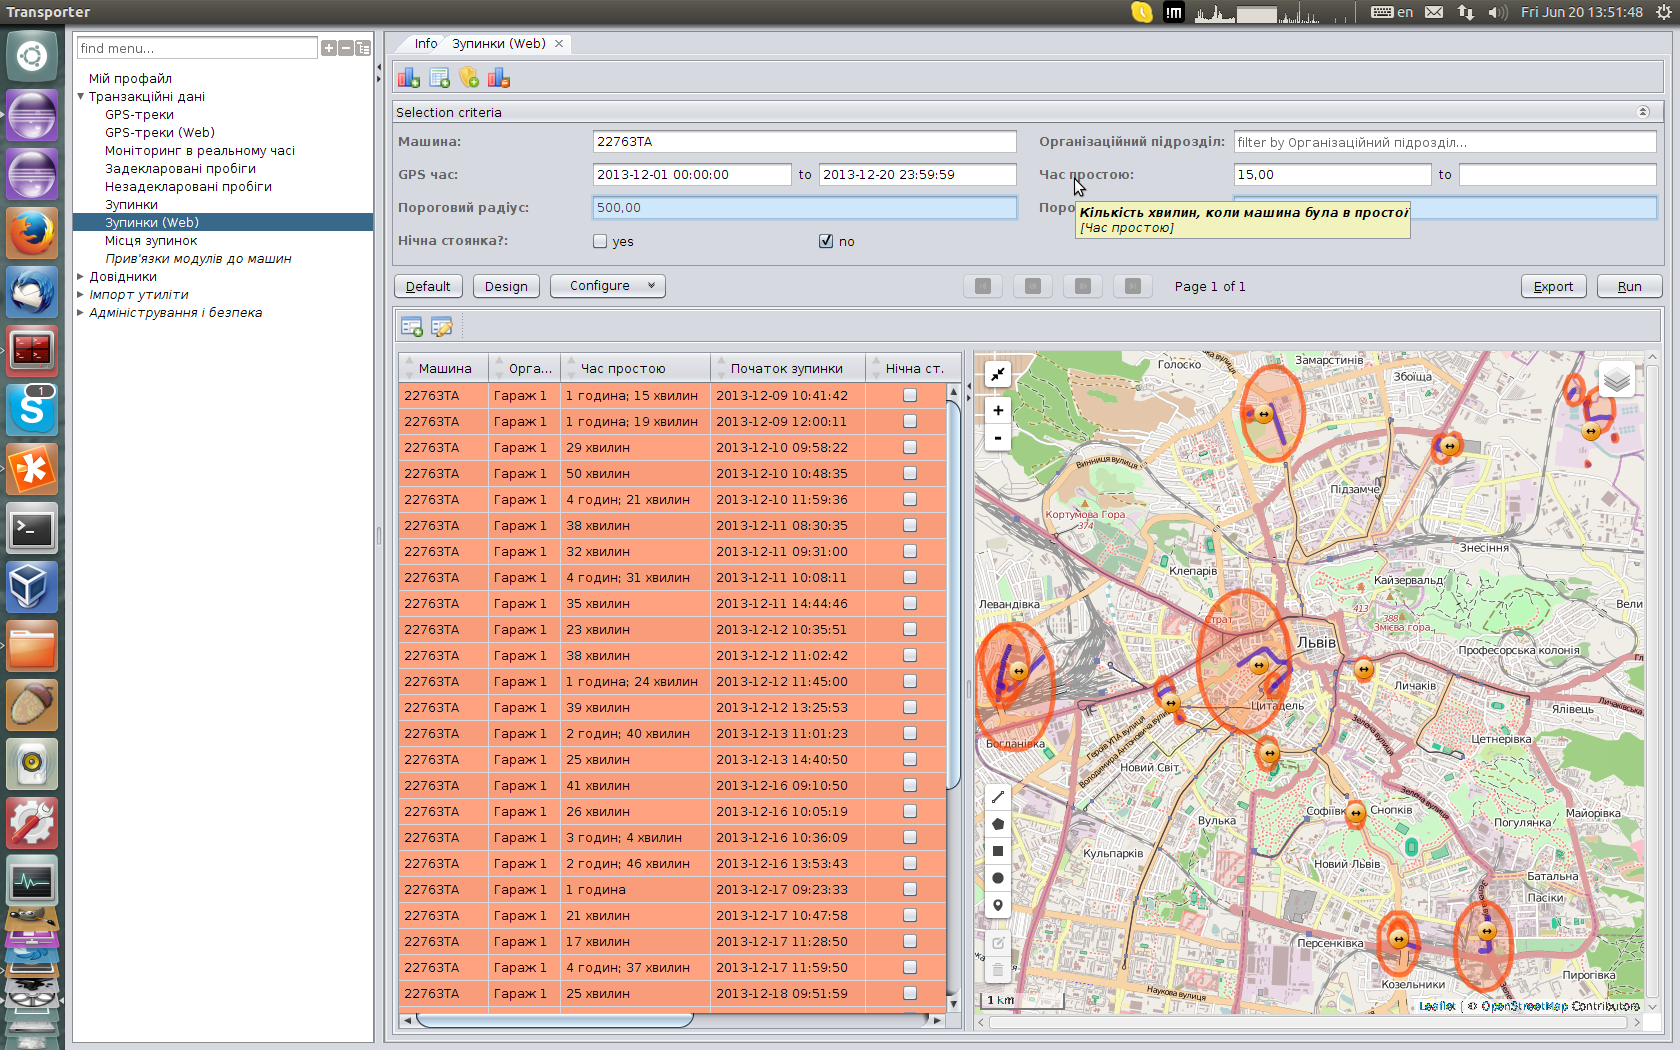
\includegraphics[width=\linewidth]{chapters/03-stoppages/images/27-determining-stoppages-with-more-than-15-minutes-duration.png}
\caption{determining-stoppages-with-more-than-15-minutes-duration}\label{fig:27}
\end{figure}